% Sources: data/sutures/{stitches,procedures}.csv and original figure captions.
\WIPsubsection{Suture Timing}
The seven main recordings contained 62 annotated stitches: 23 with 3 mm instruments and 39 with 8 mm instruments. Suture placement time was measured from pickup of the suture needle to tightening of the final throw. The interval from final knot tightening to suture cutting by the assistant (knot-to-cut interval) was recorded separately (\cref{fig:suture-phases}).

Mean suture placement time, calculated by averaging the animal-specific means, was 7.1 minutes with 3 mm instruments and 4.1 minutes with 8 mm instruments.

At the individual-suture level, pooled median needle-passage times were 121.8 seconds with 3 mm instruments and 71.3 seconds with 8 mm instruments. Median knot-tying times were 147.1 versus 123.4 seconds. The phase distributions and knot-to-cut intervals are shown in \hyperref[fig:suture-analysis]{\Cref*{fig:suture-analysis}a} and \cref{tab:suture-phases}; stitches were clustered within pigs.

Needle passage and knot tying were also summarised by annotated repair region in the \hyperref[sec:supplement]{supplement} (\cref{tab:suture-regions}). \hyperref[fig:suture-analysis]{\Cref*{fig:suture-analysis}b--c} shows throw counts and distributions of knot-tying time per throw. Both groups had a median of three throws per knot; the pooled median knot-tying time per throw was 52.6 versus 43.5 seconds (\cref{tab:knot-throws}). Per-animal statistics are reported in \cref{tab:suture-by-pig}. Motion data were available for 58 stitches and are reported separately (\cref{tab:phase-motion,tab:phase-motion-knot}).

% Single-column composite exported by the analysis repository.
\begin{figure}[!tbp]
\centering
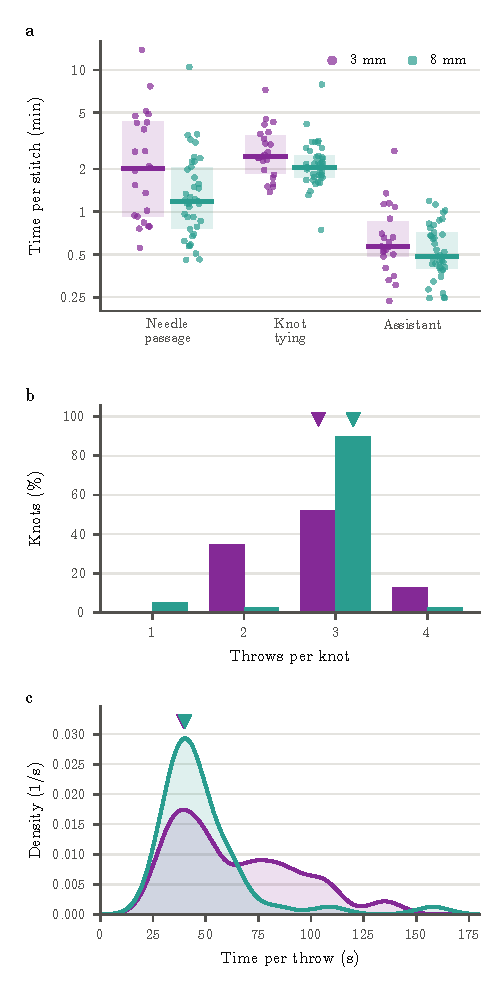
\includegraphics[width=\linewidth]{figures/results/suture_combined.pdf}
\caption{Suture timing and knot throws. (a) Needle passage, knot tying, and knot-to-cut intervals in minutes with each point representing a stitch. Shaded boxes show interquartile range with line indicating the median. (b) Throws per knot with triangle marking mode. (c) Knot-tying time per throw with triangles indicating modes of 39.4 and 40.2 seconds.}
\label{fig:suture-analysis}
% Alias labels preserve existing cross-references to the now-combined figure.
\label{fig:suture-phases}
\label{fig:knot-throws-mode}
\end{figure}

% \begin{itemize}
% \item The analysis excluded the 15.5-minute P01 final knot-to-cut interval as an outlier. Its analyzed procedure duration changed from 115.60 to 100.08 minutes.
% % Editorial: Document the exclusion rationale and sensitivity to retaining this interval.
% \item The P03 block summary included a repeated soft-palate block with 909\% stitching occupancy. Block-level occupancy was not used here.
% % Editorial: Confirm the P07 duplicate needle-through mark and report timing by comparable repair phase.
% \end{itemize}
